\documentclass{article}\usepackage[]{graphicx}\usepackage[]{color}
%% maxwidth is the original width if it is less than linewidth
%% otherwise use linewidth (to make sure the graphics do not exceed the margin)
\makeatletter
\def\maxwidth{ %
  \ifdim\Gin@nat@width>\linewidth
    \linewidth
  \else
    \Gin@nat@width
  \fi
}
\makeatother

\definecolor{fgcolor}{rgb}{0.345, 0.345, 0.345}
\newcommand{\hlnum}[1]{\textcolor[rgb]{0.686,0.059,0.569}{#1}}%
\newcommand{\hlstr}[1]{\textcolor[rgb]{0.192,0.494,0.8}{#1}}%
\newcommand{\hlcom}[1]{\textcolor[rgb]{0.678,0.584,0.686}{\textit{#1}}}%
\newcommand{\hlopt}[1]{\textcolor[rgb]{0,0,0}{#1}}%
\newcommand{\hlstd}[1]{\textcolor[rgb]{0.345,0.345,0.345}{#1}}%
\newcommand{\hlkwa}[1]{\textcolor[rgb]{0.161,0.373,0.58}{\textbf{#1}}}%
\newcommand{\hlkwb}[1]{\textcolor[rgb]{0.69,0.353,0.396}{#1}}%
\newcommand{\hlkwc}[1]{\textcolor[rgb]{0.333,0.667,0.333}{#1}}%
\newcommand{\hlkwd}[1]{\textcolor[rgb]{0.737,0.353,0.396}{\textbf{#1}}}%
\let\hlipl\hlkwb

\usepackage{framed}
\makeatletter
\newenvironment{kframe}{%
 \def\at@end@of@kframe{}%
 \ifinner\ifhmode%
  \def\at@end@of@kframe{\end{minipage}}%
  \begin{minipage}{\columnwidth}%
 \fi\fi%
 \def\FrameCommand##1{\hskip\@totalleftmargin \hskip-\fboxsep
 \colorbox{shadecolor}{##1}\hskip-\fboxsep
     % There is no \\@totalrightmargin, so:
     \hskip-\linewidth \hskip-\@totalleftmargin \hskip\columnwidth}%
 \MakeFramed {\advance\hsize-\width
   \@totalleftmargin\z@ \linewidth\hsize
   \@setminipage}}%
 {\par\unskip\endMakeFramed%
 \at@end@of@kframe}
\makeatother

\definecolor{shadecolor}{rgb}{.97, .97, .97}
\definecolor{messagecolor}{rgb}{0, 0, 0}
\definecolor{warningcolor}{rgb}{1, 0, 1}
\definecolor{errorcolor}{rgb}{1, 0, 0}
\newenvironment{knitrout}{}{} % an empty environment to be redefined in TeX

\usepackage{alltt}
\usepackage{Sweave}
\usepackage{float}
\usepackage{graphicx}
\usepackage{tabularx}
\usepackage{siunitx}
\usepackage{geometry}
\usepackage{pdflscape}
\usepackage{mdframed}
\usepackage{amssymb} % for math symbols
\usepackage{amsmath} % for aligning equations
\usepackage{natbib}
\bibliographystyle{..//refs/styles/besjournals.bst}
\usepackage[small]{caption}
\setlength{\captionmargin}{30pt}
\setlength{\abovecaptionskip}{0pt}
\setlength{\belowcaptionskip}{10pt}
\topmargin -1.5cm        
\oddsidemargin -0.04cm   
\evensidemargin -0.04cm
\textwidth 16.59cm
\textheight 21.94cm 
%\pagestyle{empty} %comment if want page numbers
\parskip 7.2pt
\renewcommand{\baselinestretch}{1.5}
\parindent 0pt
\usepackage{lineno}
\linenumbers

\newmdenv[
  topline=true,
  bottomline=true,
  skipabove=\topsep,
  skipbelow=\topsep
]{siderules}

%% R Script


\IfFileExists{upquote.sty}{\usepackage{upquote}}{}
\begin{document}
\noindent \textbf{\large{Rethinking False Spring Risk: Supplement}}

\noindent Authors:\\
C. J. Chamberlain $^{1,2}$, B. I. Cook $^{3}$, I. Garcia de Cortazar Atauri $^{4}$ \& E. M. Wolkovich $^{1,2}$
\vspace{2ex}\\
\emph{Author affiliations:}\\
$^{1}$Arnold Arboretum of Harvard University, 1300 Centre Street, Boston, Massachusetts, USA; \\
$^{2}$Organismic \& Evolutionary Biology, Harvard University, 26 Oxford Street, Cambridge, Massachusetts, USA; \\
$^{3}$NASA Goddard Institute for Space Studies, New York, New York, USA; \\
$^{4}$French National Institute for Agricultural Research, INRA, US1116 AgroClim, F-84914 Avignon, France
\vspace{2ex}
$^*$Corresponding author: 248.953.0189; cchamberlain@g.harvard.edu\\

\renewcommand{\thetable}{S\arabic{table}}
\renewcommand{\thefigure}{S\arabic{figure}}
\renewcommand{\labelitemi}{$-$}
\setkeys{Gin}{width=0.8\textwidth}

%%%%%%%%%%%%%%%%%%%%%%%%%%%%%%%%%%%%%%%%%%%%%%%

\subsection*{Defining False Spring: An example in one temperate plant community - \textit{methods for calculating FSI in Harvard Forest example}}
We collected data for determining biological spring onset using three methods for Harvard Forest. The first method for was from long-term observational data recorded for 33 tree species by John O'Keefe at Harvard Forest from 1990 to 2014 \citep{OKeefe2014}. Budburst was definied as 50\% green tip emergence. We subsetted this dataset to include only the tree species that were most consistently observed (eight species). The second dataset was from Harvard Forest's PhenoCam data, which are field cameras placed in the forest canopy that take real-time images of plant growth and are programmed to record initial green up. The final set was ``First Leaf - Spring Onset"  from the Extended Spring Index \citep[SI-X,][]{SI-x2016}, accessed via the ``Spring Indices, Historic Annual" gridded layer of the USA National Phenology Network;s (USA-NPN) Data Visualization tool. The SI-x model was built from historical budburst data from honeysuckle and lilac clones clones around the U.S. combined with daily recordings from local weather stations \citep{USA-NPN2016, Ault2015, Ault2015a, Schwartz2013, Schwartz1997}. Through assessing past years' weather and budburst, scientists are able to determine general weather trends that subsequently lead to leaf out. Based on these trends, SI-x values are calculated from daily weather data \citep{USA-NPN2016}.
% EMW: Can you check your SI-x definition? My understanding of SI is that it is *estimated* leafout (etc.) dates based on model built to well-predict lilac and honeysuckle data. I would actually refer to this in figures as SI-x (Spring Index) first leaf as opposed to NPN. The phenology community thinks of NPN as the citizen science data and the Spring Index as separate (but hosted by NPN). I think we could say all this more clearly (for example, you say 'uses the time of leaf out using historical dates of budburst,' does it really use budburst to estimate leafout? I made a few changes, but see if they are correct and try to clarify further. 
\par
The date of last spring freeze was gathered from the Fisher Meteorological Station which was downloaded from the Harvard Forest web page (data available online\footnote{http://harvardforest.fas.harvard.edu/meteorological-hydrological-stations}). The $T_{min}$ values were used and the last spring freeze was determined from the latest spring date that the temperature reached -2.2$^{\circ}$C or below. 
\par
PhenoCam data are not available for Harvard Forest until 2008 and observation data is only recorded through 2014, so this evaluation assesses FSI values from 2008 through 2014.
\par The FSI values were calculated for each methodology using the formula based on the study performed by Marino et al. (2011).  

\subsection*{How Species' Phenological Cues Shape Vegetative Risk - \textit{methods for experiment}}
We used data from a growth chamber experiment (Flynn2018) to assess the phenological cue interaction with the duration of vegetative risk. Cuttings for the experiment were made in January 2015 at Harvard Forest (HF, 42.5$^{\circ}$N, 72.2$^{\circ}$W) and the Station de Biologie des Laurentides in St-Hippolyte, Qu\'ebec (SH, 45.9$^{\circ}$N, 74.0$^{\circ}$W). The experiment considered here examined the 9 temperate trees and shrubs used in a fully crossed design of three levels of chilling (field chilling, field chilling plus 30 days at either 1 or 4 $^{\circ}$C), two levels of forcing (20$^{\circ}$C/10$^{\circ}$C or 15$^{\circ}$C/5$^{\circ}$C day/night temperatures, such that thermoperiodicity followed photoperiod) and two levels of photoperiod (8 versus 12 hour days) resulting in 12 treatment combinations. Observations on the phenological stage of each cutting were made every 2-3 days over 82 days. Phenology was assessed using a BBCH scale that was modified for trees \citep{Finn2007}. We used the same statistical analyses as the original study: mixed-effects hierarchical models that included warming, photoperiod, and chilling treatments, and all two-way interactions as predictors and species modeled as groups.

The model equation is as from the original study:
\begin{align*}
y_i \thicksim N(\alpha_{sp[i]} +& \beta_{site_{sp[i]}} + \beta_{forcing_{sp[i]}} + \beta_{photoperiod_{sp[i]}} + \beta_{chilling1_{sp[i]}} + \beta_{chilling2_{sp[i]}}  \\
	+& \beta_{forcing \times photoperiod_{sp[i]}} + \beta_{forcing \times site_{sp[i]}} + \beta_{photoperiod \times site_{sp[i]}} \\
	+& \beta_{forcing  \times chilling1_{sp[i]}} + \beta_{forcing \times chilling2_{sp[i]}} \\
	+& \beta_{photoperiod \times chilling1_{sp[i]}} + \beta_{photoperiod \times chilling2_{sp[i]}} \\
	+& \beta_{site \times chilling1_{sp[i]}}  + \beta_{site \times chilling2_{sp[i]}} )
\end{align*}

\noindent And the $\alpha$ and each of the 14 $\beta$ coefficients were modeled at the species level in the original study, as follows:
\begin{align*}
1.& \; \beta_{site_{sp}} \thicksim N(\mu_{site}, \sigma{^2}_{site}) \\
   &... \\
14.& \; \beta_{site \times chilling2_{sp}} \thicksim N(\mu_{site \times chilling2}, \sigma{^2}_{site \times chilling2})
\end{align*}

\subsection*{Predictable Regional Differences in Climate, Species Responses and False Spring Risk - \textit{climate data and phenology data}}
%EMW: Include changes from above here below!
We analyzed five archetypal regions across North America and Europe. We collected phenology data through the USA National Phenology Network (USA-NPN), using their Data Visualization tool to gather Extended Spring Index values (SI-x) by accessing the ``Spring Indices, Historic Annual" gridded layer and looking specifically at ``First Leaf - Spring Onset" \citep{SI-x2016}. We looked at each SI-x value for each North American site (i.e. Waterville, ME, Yakima, WA, and Reidsville, NC) from 1981-2016 to evaluate the spread of spring onset dates for those regions. For the European sites (i.e. Bamberg, Germany and Lyon, France) we used phenology observation studies that assessed multiple years of \textit{in situ} budburst to leafout dates for the dominant species in those regions \citep{Soudani2012, White2009,Schaber2005}. We then collected climate data by downloading Daily Summary climate datasets from the NOAA Climate Data Online tool (data available online\footnote{https://www.ncdc.noaa.gov/cdo-web/search?datasetid=GHCND}). We gathered 50 years of climate data for each location from NOAA, then calculated the number of years that fell below -2.2$^{\circ}$C within the budburst to leafout date range for each region. % EMW: These methods don't full agree with the caption or I could easily be missing something, but here you seem to refer to budburst only and in the caption you say between budburst and leafout. Make the two agree. 

\newpage
\subsection*{Supplemental Figures}
\begin{figure} [H] 
 \begin{center}
 %\textbf{Regional Differences in False Spring Risk}\par\medskip
 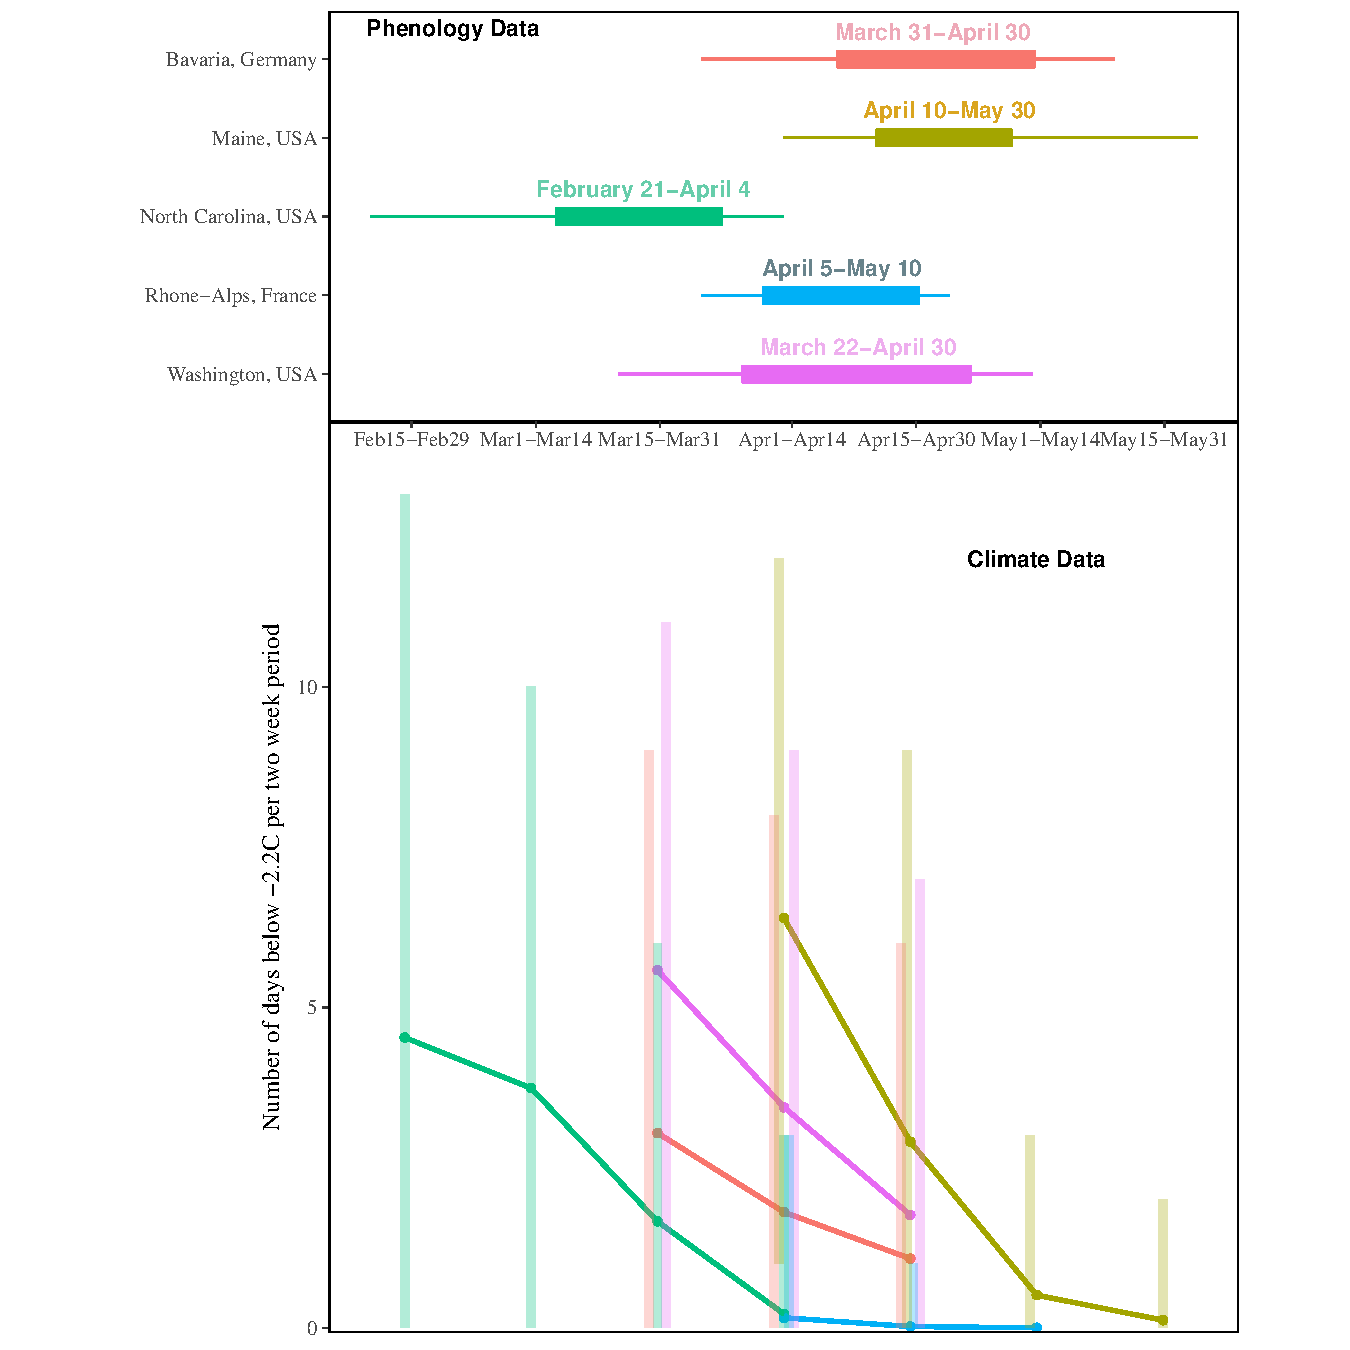
\includegraphics[width=16cm, height=18cm]{..//figure/RegRisk_flipped.pdf} 
 \caption{False spring risk can vary dramatically across regions. Here we show the period when plants are most at risk to tissue loss -- between budburst and leafout (upper, lines represent the range with the thicker line representing the interquartile range) and the variation in the number of freeze days (-2.2$^{\circ}$C) (Schwartz, 1993) that occurred on average over the past 50 years for five different sites (lower, bars represent the range, points represent the mean). Data come from USA-NPN SI-x tool (1981-2016) and observational studies (1950-2016) for phenology (USA-NPN, 2016; Soudani et al., 2012; White et al., 2009; Schaber \& Badeck, 2005) and NOAA Climate Data Online tool for climate (from 1950-2016). } \label{fig:regional}  
 \end{center}
 \end{figure}


\newpage
\nocite{Flynn}
\bibliography{..//refs/SpringFreeze.bib}

\end{document}
